%!xelatex = 'xelatex --halt-on-error %O %S'

\documentclass{buaaemp}
\begin{document}

% 标题,作者
\emptitle{单边pn结杂质分布的锁相检测}
\empauthor{智朝晖}{蔡微}

% 奇数页页眉 % 请在这里写出第一作者以及论文题目
\fancyhead[CO]{{\footnotesize 智朝晖: 单边pn结杂质分布的锁相检测}}


%%%%%%%%%%%%%%%%%%%%%%%%%%%%%%%%%%%%%%%%%%%%%%%%%%%%%%%%%%%%%%%%
% 关键词 摘要 首页脚注
%%%%%%%%关键词
\Keyword{杂质分布, C-V法, 锁相放大, 自建势}
\twocolumn[
\begin{@twocolumnfalse}
\maketitle

%%%%%%%%摘要
\begin{empAbstract}
本文利用EG&G公司生产的DSP7265型锁相放大器,通过测量不同直流偏压下p-n结势垒电容的方法(C-V法)来求得杂质浓度的分布,并且计算得到p-n结的自建势。
\end{empAbstract}

%%%%%%%%首页角注,依次为实验时间、报告时间、学号、email
\empfirstfoot{2022-10-27}{2022-10-27}{20377365}{20377365@buaa.edu.cn}
\end{@twocolumnfalse}
]
%%%%%%%%!首页角注可能与正文重叠,请通过调整正文中第一页的\enlargethispage{-3.3cm}位置手动校准正文底部位置:
%%%%%%%%%%%%%%%%%%%%%%%%%%%%%%%%%%%%%%%%%%%%%%%%%%%%%%%%%%%%%%%%
%  正文由此开始
\wuhao 
%  分栏开始

\section{引~~言}
\mathrm{p}-\mathrm{n}  结的杂质分布对半导体器件 (如光敏二极管、LED 等) 的特性有很大影响, 控制 p-n 结的杂质分布是制造半导体器件的重要课题。检测 p-n 结的杂质分布对改进制造工 艺, 了解器件性能是必要的。通过测量不同反向偏值电压下的  \mathrm{p}-\mathrm{n}  结势垒电容, 可以方便 地测得单边突变  p-n  结轻掺杂一边的杂质浓度及分布。
锁定放大器(Lock-in Amplifier)是一种用相干检测方法测量微弱信号的检测仪器。 它能在强噪声背景下, 提取周期信号的幅度和相位值, 但不能复现信号的波形。微弱信 号测量就是要克服背景噪声, 提取有用信号。\cite{钱建强2016近代物理实验}


\section{原~~理}
\subsection{p-n结势垒电容与杂质浓度的关系}
当  p-n  结一边的杂质比另一边浓得多, 即 $ N_{A} \gg>N_{D} $ 。 $ N_{A}$  是受主杂质密度, 对应  p  型半 导体; $ N_{D} $ 是施主杂质密度, 对应  $\mathrm{n}$  型半导体。这样的 $ \mathrm{p}-\mathrm{n} $ 结为单边突变结, 浅扩散法常 用它作近似。

单边突变结的  n  边和  p  边宽度关系为  $x_{n}>>x_{p}$ , 因此, 总空间电荷区的宽度 $ \mathrm{w} \approx \mathrm{x}_{\mathrm{n}}$  。如图\ref{fig:fig1}即电势的变化几乎都落到轻掺杂的 $ \mathrm{n}$  区, 而重掺杂一边的  $\mathrm{p}$  区可以忽略。这样, 空间电荷区宽度和偏压 $ V_{R} $ 的关系仅与轻掺杂浓度  $N_{D}$  有关
\newpage

\begin{equation*}
    w=\sqrt{\frac{2 \varepsilon \varepsilon_{0}}{q N_{D}}\left(V_{D}+V_{R}\right)}
\end{equation*}

\begin{figure}
    \centering
    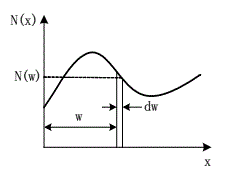
\includegraphics{image/杂质分布.png}
    \caption{轻掺杂区的杂质分布}
    \label{fig:fig1}
\end{figure}
其中  $\varepsilon$  为相对介电常数, 对于硅 $ \varepsilon=11.8, \varepsilon_{0}$  是真空介电常数,  q  为电子电荷,  $V_{D}$  是  $\mathrm{p}-\mathrm{n}  $结的接触电势差。这时, p-n 结每一边的存则的电荷 $ \mathrm{Q}$  与空间电荷区宽度 $ \mathrm{w}  $成正比

\begin{equation*}
    Q A=q A N_{D} w=A \sqrt{2 q \varepsilon \varepsilon_{0}\left(V_{D}+V_{R}\right) N_{D}}
\end{equation*}

其中  $\mathrm{A}$  为 $ \mathrm{p}-\mathrm{n}$  结的结面积。单位面积的  $\mathrm{p}-\mathrm{n} $ 结势垒电容
\begin{equation*}
    \frac{C}{A}=\frac{d Q}{d V_{R}}=\sqrt{\frac{q \varepsilon \varepsilon_{0} N_{D}}{2\left(V_{D}+V_{R}\right)}}=\frac{\varepsilon \varepsilon_{0}}{w}
\end{equation*}


上式表明, 当偏压改变量  $\Delta V_{R}  $足够小时, 空间电荷区的电荷改变量  A $\Delta Q $ 与  $\Delta V_{R}$  成 正比, 其比值即为 $ \mathrm{p}-\mathrm{n} $ 结势垒电容  $\mathrm{C} $ 。这和一个平行板电容器有相似之处, 电容值正比于  p-n  结的结面积  A , 反比于空间电荷区的宽度  w  。当  p-n  结上外加偏压增加  $\Delta V_{R}$  时, 空间 电荷区的宽度将增加  $\Delta \mathrm{w}$ , 原来在这  $\Delta \mathrm{w}$  层内的载流子  ($\mathrm{n}$  区的电子,  $\mathrm{p} $ 区的空穴)将流 走, 形成放电电流, 使空间电荷量增加 $ A \Delta Q$  。而当偏压减小  $\Delta V_{R} $ 时, 通过放电电流使 载流子填充到 $ \Delta \mathrm{w}$  层内, 分别中和  $\mathrm{n}$  区这一层的电离失主的正电荷和$  \mathrm{p}$  区这一层的的电离 受主的负电荷, 使空间电荷区减小 $ \Delta \mathrm{w} $, 空间电荷量减少  $\mathrm{A} \Delta \mathrm{Q}$  。微量的充放电电荷  $\mathrm{A} \Delta \mathrm{Q}$  集中在空间电荷区两边的薄层 $ \Delta \mathrm{w}$  内, 这两个薄层相当于相距  $\mathrm{w} $ 的两个平行极板,半导体本身构成了电容器的介质。但是 p-n 结势垒电容与平行板电容也有区别, 主要在于 空间电荷区宽度 $ \mathrm{w}$  与平行板电容器的极间距离不同,  $\mathrm{w} $ 是随外加偏压的变化而改变。因 此, p-n 结势厽电容也是随外加偏压的变化而改变。正是由于这个特点, 通常也把 p-n 结 势垒电容称为微分电容。将式  改写为
\begin{equation*}
    \frac{2}{C^{2}}=\frac{2}{A^{2} q \varepsilon \varepsilon_{0} N_{D}}\left(V_{D}+V_{R}\right)
\end{equation*}


作出$  1 / \mathrm{C}^{2} \sim \mathrm{V}_{\mathrm{R}} $ 曲线一一直线, 由其斜率可以计算施主杂质浓度 $ \mathrm{N}_{\mathrm{D}}  $。将直线外推到电 压轴, 可以求出接触电势差 $ V_{D}$  。
对于一个末知杂质分布的  $\mathrm{p}-\mathrm{n}  $结, 可以利用  $\mathrm{p}-\mathrm{n} $ 结电容一电压曲线描绘出轻掺杂一边 的杂质分布。图 1 表示一个  $\mathrm{p}^{+} \mathrm{n}$  结在  $\mathrm{n}  $区有一个任意的杂质分布。当空间电荷区宽度变化  $\mathrm{dw} $ 时, 相应的单位面积的空间电荷变化量

$$d Q=q N(w) d w$$

其中  $\mathrm{N}(\mathrm{w})  $是空间电荷区宽度 $ \mathrm{w}$  边界处的杂质浓度。
增加的电荷$  \mathrm{dQ}$  引起电场改变  $\mathrm{dE} $
相应的电势改变$  \mathrm{dV}$ 

\begin{equation*}
    d E=\frac{d Q}{\varepsilon \varepsilon_{0}}
\end{equation*}

由上两式得到
\begin{equation}
    \frac{dQ}{dV_{R}}=\frac{\epsilon \epsilon_0}{w}=\frac{C}{A} \label{equ1}
\end{equation}
 整理后得到

\begin{equation*}
    N(w)=\frac{2}{q \varepsilon \varepsilon_{0} A^{2}} \cdot \frac{1}{\frac{d\left(1 / C^{2}\right)}{d V_{R}}}
\end{equation*}

由上式可知, 测量出 $ \mathrm{p}-\mathrm{n}$  结势垒电容 $ \mathrm{C}  $其偏压变化后, 作出 $ 1 / \mathrm{C}^{2} \sim \mathrm{V}_{\mathrm{R}} $ 曲线, 并求出 各偏压下的 $ \mathrm{d}\left(1 / \mathrm{C}^{2}\right) / \mathrm{dV}_{R} $, 代入上式, 就能得到$  \mathrm{N}(\mathrm{w})$  。上式也可改写成

\begin{equation*}
    N(w)=-\frac{1}{q \varepsilon \varepsilon_{0} A^{2}} \cdot \frac{C^{3}}{d C / d V_{R}}
\end{equation*}

采用直接求 $ \mathrm{C} \sim \mathrm{V}$  曲线在不同偏压下的斜率 $ \mathrm{dC} / \mathrm{dV} \mathrm{R}_{\mathrm{R}}$ , 并将该偏压下的 $ \mathrm{p}-\mathrm{n}$  结电容 $ \mathrm{C}$ 一  同代入上式, 也能得到 $ \mathrm{N}(\mathrm{w}) $ 。此外, 由式\ref{equ1}可以通过电容确定不同偏压下所对应的  p-n  结空间电荷区宽度  w 。 N(w)  是距离  p-n  结交界处  (x=0)  的杂质浓度。 $ N(w) \sim W$  就是所 要确定的杂质分布。以上方法适合求出扩散法和离子注入法产生的杂质分布。
\subsection{C-V关系测量原理}\cite{钱建强2016近代物理实验}
 p-n  结势垒电容是一个随直流偏压变化的微分电容。测量势垒电容时, 首先要在 p-n 结上加上反向偏置电压 $ \mathrm{V}_{\mathrm{R}}$  。再将一个幅度远小于  $\mathrm{V}_{\mathrm{R}}$  的正弦信号$  v_{0}(t) $ 叠加到 $ \mathrm{p}-\mathrm{n} $ 结上。 由于电容$  \mathrm{C}_{1}>\mathrm{C}_{\mathrm{x}} $, 通过  $\mathrm{C}_{1} $ 和  $\mathrm{C}_{\mathrm{x}}$  的交流电流幅度值主要取决 $ \mathrm{C}_{\mathrm{x}} $, 落到 $ \mathrm{C}_{1} $ 上的交 流电压为

\begin{equation}
    v_{1}(t) \approx I(t) \cdot \frac{1}{j \omega C_{1}}=\frac{v_{0}(t)}{\frac{1}{j \omega C_{x}}} \cdot \frac{1}{j \omega C_{1}}=\frac{C_{x}}{C_{1}} v_{0}(t) \label{equ2}
\end{equation}

其中 $ 1 / j \omega C $ 为电容的复阻抗。注意, 直流偏压经过一个 $ 100 \mathrm{~K} \Omega $ 电阻接到被测器件 $ \mathrm{A}$  极, 与 $ \mathrm{C}_{1}$  的阻抗相比, 这个电阻可视为断路;  $\mathrm{C}_{1}$  的值不能选得过小, 否则不能用式\ref{equ2} 计算  $v_{1}(t)$  的幅度。另外, 锁定放大器输入端阻抗近似于无穷大。
根据式\ref{equ2}, 在已知 $ \mathrm{C}_{1}$  时, 只要测出  $v_{0}(t) $ 和  $v_{1}(t)$  的幅度值, 就能求出 $ \mathrm{C}_{\mathrm{x}}$  。 如果正弦信号  $v_{0}(t) $ 的幅度值过大, 会引起 p-n 结电容出现变化, 带来测量误差, 因 此应尽量小些, 可选  $30 \mathrm{mV} $ 左右。这样 $ v_{1}(t) $ 的幅度  $\mathrm{V}_{1}$  就会很小, 因此, 本实验采用锁定 放大器来测量这个幅度值。

\subsection{锁相放大器的噪声和频带}
锁定放大器(Lock-in Amplifier)是一种测量微弱信号的检测仪器。微弱信号测量就 是要克服背景噪声, 提取有用信号。为此, 首先需要了解噪声的特点。

传感器在将被测物理量转换为电信号时, 都不可避免地带进些 “噪声”。这些噪声 包括: 传感器本身的噪声, 测量仪表仪器的噪声, 以及其它随即误差。在微弱信号测量 中, 电子器件如包括传感器和放大电路, 产生的电子噪声是影响测量结果的关键因素。 电子噪声主要有
热噪声:任何电子器件, 其中总有导电的载流子, 在一定温度下, 这些载流子作不 规则的热运动, 使器件中的载流子定向流动出现起伏, 形成热噪声电流。热噪声的有效 值和系统的频宽的方根成正比。在相同的频宽下, 无论频率的高低, 热噪声的强度都是 相同的。简单的说, 在一定范围内, 噪声功率有效值与系统频宽的方根成正比, 与频率 无关, 称为白噪声。另外, 温度越高, 热噪声越强。粒噪声:即使进入探测器光强,在宏观上是稳定的,但从光的量子特性可知,相等 的时间内,进入探测器的光子数是会涨落的:传感器的转换效率 (量子效率) 实际是是 有起伏变化的;测量时载流子数目的起伏。都会产生散粒噪声。散粒噪声也是白噪声。
电流噪声: 电传感器在没有信号输入时,往往也有电流输出,称为暗电流。它的产 生机理随器件而异。暗电流噪声也是白噪声。
频噪声:因器件材料中的晶体缺陷等产生的噪声。它与频率的倒数 $ 1 / \mathrm{f}$  及频率成正 比,又称为  $1 / \mathrm{f} $ 噪声。频率越低 $ 1 / \mathrm{f} $ 噪声越大, 在 $ 1000 \mathrm{~Hz} $ 以下有较大影响。
可见以各种噪声可以通过限制频带宽度, 使有用的信号通过, 大幅度降低噪 声。在信噪比不过低时, 往往采用窄带滤波器或选频放大器, 放大信号、抑制噪声。滤 波 器的性能用带宽  $\Delta \mathrm{f}$  和中心频率 $ \mathrm{f}_{0}$  来描述。一般带宽 $ \Delta \mathrm{f}$  不可能作得很窄;  $\mathrm{f}_{0}$  也不是十 分稳定, 这就需要加大带宽, 降低了对噪声的抑制。对于微弱信号的检测, 使用窄带滤 波的方法往往不能满足要求。
\subsection{米检测和相关器}
相关检测技术利用信号周期性和噪声随机性的特点,即信号在时间轴上前后相关, 噪声与信号互不相关, 通过相关运算提取信号, 去除噪声
设信号 $ f_{1}(t)  和  f_{2}(t-\tau) $, 其相关函数定义为
\begin{equation*}
     R(\tau)=&\lim _{\tau \rightarrow \infty} \frac{1}{2 T} \int_{-T}^{T}f_1(t)f_2(t-\tau)dt
\end{equation*}

设 $f_1(t)=V_S(t)+n_1(t) \  f_2(t)=V_R(t)+n_2(t)$

其中 $V_S$为被测信号, $V_R$为参考信号 $n_S(t) n_R(t)$为伴随的噪声。带入上式:

\begin{aligned}
      R(\tau)=&\lim _{\tau \rightarrow \infty} \frac{1}{2 T}\int_{-T}^{T} (V_{S}(t)+n_1(t))( V_{R}(t-\tau)+n_2(t-\tau)) d t  \\
     &=R_{S R}(\tau)+R_{S 2}(\tau)+R_{R 1}(\tau)+R_{12}(\tau) 
\end{aligned}

其中 $ R_{S R}(\tau), R_{S 2}(\tau), R_{R 1}(\tau), R_{12}(\tau)$  
分别为信号之间、信号与噪声之间和噪声之间的相关函数。由于噪声的随机性噪声之间以及和信号之间的相关函数在积分时 间足够长时, 应为零,也即抑制了噪声。
完成相关检测的仪器叫做相关器, 主要由乘法器和积分器 组成。乘法器分为模拟乘法器和开关式乘法器两种, 现多采用后者。积分器实际使用多 阶有源低通滤波器。 如果被测信号表示为:  $V_{S} \cos \left(\omega_{S} t+\theta_{S}\right)$ , 参考信号表示为:  $V_{R} \cos \left(\omega_{R} t+\theta_{R}\right)$ , 这 两个信号通过乘法器相乘,乘法器的输出为

\begin{aligned}
V_{X} &=V_{S} V_{R} \cos \left(\omega_{S} t+\theta_{S}\right) \cos \left(\omega_{R} t+\theta_{R}\right) \\
&=\frac{1}{2} V_{S} V_{R} \cos \left[\left(\omega_{S}-\omega_{R}\right) t+\left(\theta_{S}-\theta_{R}\right)\right]+ \\
&\frac{1}{2} V_{S} V_{R} \cos \left[\left(\omega_{S}+\omega_{R}\right) t+\left(\theta_{S}+\theta_{R}\right)\right] \label{equ3}
\end{aligned}

由上式可知, 乘法器的输出是两个交流信号, 即一个是差频项 $ \omega_{S}-\omega_{R} $, 另一个是 和频项$  \omega_{S}+\omega_{R}$ , 乘法器的输出信号经过低通滤波器, 和频项信号被消除。当被测信号 和参考信号频率相同时, 差频项信号的成分变为直流信号

$$V_{X}=\frac{1}{2} V_{S} V_{R} \cos \left(\theta_{S}-\theta_{R}\right)$$

这个直流信号既是我们需要测量的信号。
由式\ref{equ3} 可知, 在被测信号和参考信号频率相同的情况下, 乘法器经低通滤波器 的输出只与输入信号和参考信号的相位差有关。如果输入信号与参考信号的相位差为 零, 即  $\theta=\theta_{S}-\theta_{R}=0 $ ,
则 $ V_{X}=\frac{1}{2} V_{S} V_{R}$  。由此, 可 以得到这样的结果: 当输入 信号与参考信号的相位同相 (或反相) 时, 乘法器经低 乘法器 通滤波器输出的直流电压最
 $\frac{1}{2} V_{s} V_{R} \cos \left(\theta_{s}-\theta_{R}\right)$  大。

其结构如图\ref{fig:fig2}
\begin{figure}
    \centering
    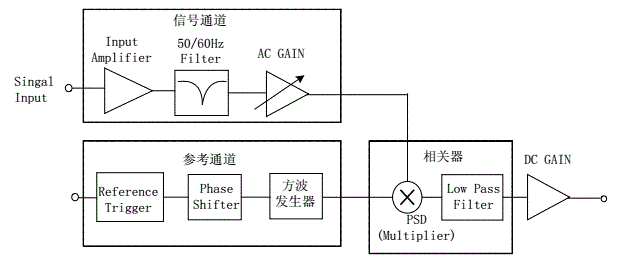
\includegraphics[width=\linewidth]{image/锁相放大器.png}
    \caption{锁相放大器原理框图}
    \label{fig:fig2}
\end{figure}

\section{实~~验}
实验步骤如下:

1. 仔细阅读锁定放大器的说明书, 结合仪器, 熟悉面板操作。

2. 连接实验电路。

3. 将信号发生器 “Ampl” 钮逆时针调到头。开信号发生器电源。将频率调整到  10000 \mathrm{~Hz}  。调整 “Ampl” 钮, 使毫伏表指示  20 \mathrm{mV}  。

4. 开锁相放大器, 检查各项设置,调节界面显示信号的频率、初相、振幅。

5. 调整锁定放大器, 到实验室指定的要求。

6. 逐点法测量  \mathrm{V}_{1} \sim \mathrm{V}_{\mathrm{R}}  关系曲线, 间隔  \Delta \mathrm{V}_{\mathrm{R}}  为  0.1 \mathrm{~V}  

\section{实验结果与分析}
本实验实验数据如下:

\begin{table}[h]
\centering
\captionnamefont{\wuhao\bf\heiti}
\captiontitlefont{\wuhao\bf\heiti}
\caption{测得 $v_i$有效值} \label{tab:eg1}
\liuhao
\begin{tabular}{ccc}
\toprule
  &$v_i /mV$ &  \space  \\
\midrule 
1.159 & 1.185 &1.208\\
1.242 &1.269 &1.307 \\
 1.355 & 1.411 & 1.473\\
 1.550 & & \\
\bottomrule
\end{tabular}
\end{table}

\begin{table}[h]
\centering
\captionnamefont{\wuhao\bf\heiti}
\captiontitlefont{\wuhao\bf\heiti}
\caption{测得 $v_D$有效值} \label{tab:eg2}
\liuhao
\begin{tabular}{ccc}
\toprule
  &$v_D /V$ &  \space \\
\midrule 
6.97 & 6.48 &6.03\\
5.47 &4.99 &4.48 \\
 3.53 & 3.38 &2.98\\
 2.47 & & \\
\bottomrule
\end{tabular}
\end{table}

另外测得 $V_t$峰值590mV,即振幅208.6mV,锁相检测有效值为204.2mV,取平均值为206.4mV。串联所用二极管为IN5401 MIC,电容为6.582nF,pn结面积为$0.2mm^2$。

最后计算得到的回归曲线为:

\begin{equation}
    \frac{1}{v_i^2}=aV_R+b
\end{equation}

得到a=69941, b=264871,r=0.9826
计算得到杂质浓度分布 $N_D=9.54\times 10^{13} cm^{-3} $,得到的自建势为 $V_D=3.78mV$
\section{思考题}
\begin{itemize}
    \item 一边的掺杂浓度远高于另一边的掺杂浓度的单边突变pn结
    \item 是因为单边突变的浓度不一样导致的自建势不一样,最终导致的 $\phi \sim V_R$不一样
    \item 锁相放大器由信号通道、参考通道和相关检测器构成,核心部分是相敏检测器(PSD),框图如图\ref{fig:fig2}所示。
\end{itemize}
\section{结~~论}
本文利用EG&G公司生产的DSP7265型锁相放大器,通过测量不同直流偏压下p-n结势垒电容的方法(C-V法)来求得杂质浓度的分布 $N_D=9.54\times 10^{13} cm^{-3} $,并且计算得到p-n结的自建势$V_D=3.78mV$。


%%%%%%%%%%%%%%%%%%%%%%%%%%%%%%%%%%%%%%%%%%%%%%%%%%%%%%%%%%%%%%%%
%  参考文献
%%%%%%%%%%%%%%%%%%%%%%%%%%%%%%%%%%%%%%%%%%%%%%%%%%%%%%%%%%%%%%%%
%  参考文献按GB/T 7714-2015《文后参考文献著录规则》的要求著录. 
%  参考文献在正文中的引用方法:\cite{bib文件条目的第一行}

\renewcommand\refname{\heiti\wuhao\centerline{参考文献}\global\def\refname{参考文献}}
\vskip 12pt

\let\OLDthebibliography\thebibliography
\renewcommand\thebibliography[1]{
  \OLDthebibliography{#1}
  \setlength{\parskip}{0pt}
  \setlength{\itemsep}{0pt plus 0.3ex}
}

{
\renewcommand{\baselinestretch}{0.9}
\liuhao
\bibliographystyle{gbt7714-numerical}
\bibliography{./TempExample}
}


\end{document}
